\documentclass[10pt]{report}

\usepackage{stan-talks}

\begin{document}

\sf
\vspace*{6pt}
\noindent
\spc{\huge\bfseries \color{MidnightBlue}{Section 3.}
\\[8pt]
\spc{\Huge\bfseries \color{MidnightBlue}{Monte Carlo Methods}}}
\vfill
\noindent
\spc{\large\bfseries Bob Carpenter}
\\[4pt]
\spc{Columbia University}
\vfill
\hfill 

\mypart{Part I}{Monte Carlo \\[8pt]\spc Integration}

\sld{Monte Carlo Calculation of $\pi$}

\noindent
\begin{minipage}[t]{0.65\textwidth}\small
\vspace*{2pt}
\begin{itemize}
\item Computing $\pi = 3.14\ldots$ via simulation is \emph{the} textbook application
of Monte Carlo methods.
\vfill
\item Generate points uniformly at random within the square
\item Calculate proportion within circle ($x^2 + y^2 < 1$) and multiply by square's area (4) to produce the area of the circle.
\item This area is $\pi$ (radius is 1, so area is $\pi r^2 = \pi$)
\end{itemize}
\end{minipage}
%
\begin{minipage}[t]{0.34\textwidth}
\vspace*{12pt}
\hfill 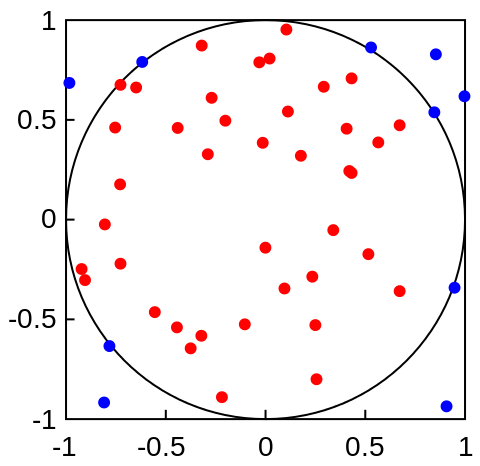
\includegraphics[height=1in]{img/mc-integration-wikipedia.png}
\\
\end{minipage}
\vfill
{ } \hfill {\tiny Plot by Mysid Yoderj courtesy of Wikipedia.}

\sld{Monte Carlo Calculation of $\pi$ {\normalsize (cont.)}}
%
\begin{itemize}
\item R code to calcuate $\pi$ with Monte Carlo simulation:
\\[-8pt]
{\small
\begin{Verbatim}
> x <- runif(1e6,-1,1)
> y <- runif(1e6,-1,1)

> prop_in_circle <- sum(x^2 + y^2 < 1) / 1e6

> 4 * prop_in_circle
[1] 3.144032
\end{Verbatim}
}
\end{itemize}

\sld{Accuracy of Monte Carlo}
\begin{itemize}
\item Monte Carlo is \emph{not} an approximation!
\item It can be made exact to within any $\epsilon$
\item Monte Carlo draws are i.i.d. by definition
\item Central limit theorem: expected error decreases at rate of
{\Large
\[
\frac{1}{\sqrt{N}}
\]
}
\item 3 decimal places of accuracy with 
sample size 1e6
\item Need $100 \times$ larger sample for each digit of accuracy
\end{itemize}

\sld{General Monte Carlo Integration}
\begin{minipage}[t]{0.69\textwidth}
\vspace*{-0.1in}
\small
\begin{itemize}
\item MC can calculate arbitrary definite integrals,
\[
\int_a^b f(x) \, dx
\]
\item Let $d$ upper bound $f(x)$ in $(a,b)$;  tightness determines
computational efficiency
\item Then generate random points uniformly in the rectangle bounded by $(a,b)$ and $(0,d)$
\item Multiply proportion of draws $(x,y)$ where $y < f(x)$ by area of rectangle, $d \times (b-a)$.
\item Can be generalized to multiple dimensions in obvious way
\end{itemize}
\end{minipage}
\begin{minipage}[t]{0.29\textwidth}
\mbox{ } \\
\mbox{ } \ \ \ \ 
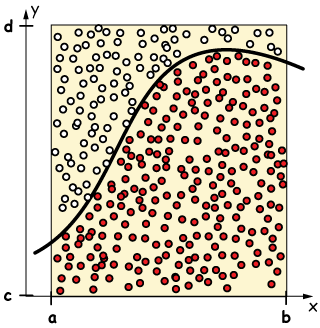
\includegraphics[height=0.9in]{img/monte-carlo-integration.png}
\end{minipage}
\vfill
\hfill
{\tiny Image courtesy of Jeff Cruzan, \url{http://www.drcruzan.com/NumericalIntegration.html}}

\sld{Expectations of Function of R.V.}
\begin{itemize}
\item Suppose $f(\theta)$ is a function of random variable vector
  $\theta$
\item Suppose the density of $\theta$ is $p(\theta)$
\begin{subitemize}
\item {\slshape Warning}: $\theta$ overloaded as random and bound variable
\end{subitemize}
\item Then $f(\theta)$ is also random variable, with expectation
  \[
  \mathbb{E}[f(\theta)] = \int_{\Theta} f(\theta) \ p(\theta) \ d\theta.
  \]
\begin{subitemize}
\item
where $\Theta$ is support of $p(\theta)$ (i.e., $\Theta =
\setcomp{\theta \, | \, p(\theta) > 0}$
\end{subitemize}
\end{itemize}

\sld{QoI as Expectations}
\begin{itemize}
\item Most Bayesian quantities of interest (QoI) are expectations
  over the posterior $p(\theta \, | \, y)$ of functions $f(\theta)$
\item \myemph{Bayesian parameter estimation}: $\hat{\theta}$
\begin{subitemize}
\item $f(\theta) = \theta$
\item $\hat{\theta} = \mathbb{E}[\theta | y]$ minimizes expected
  square error
\end{subitemize}
\item \myemph{Bayesian parameter (co)variance estimation}:
  $\mathrm{var}[\theta \, | \, y]$
\begin{subitemize}
\item $f(\theta) = (\theta - \hat{\theta})^2$
\end{subitemize}
\item \myemph{Bayesian event probability}:  $\mbox{Pr}[A \, | \, y]$
\begin{subitemize}
  \item $f(\theta) = \mathrm{I}(\theta \in A)$
\end{subitemize}
\end{itemize}



\sld{Expectations via Monte Carlo}

\begin{itemize}
\item Generate draws $\theta^{(1)}, \theta^{(2)}, \ldots,
  \theta^{(M)}$ drawn from $p(\theta)$
\item Monte Carlo Estimator \myemph{plugs in average} for expectation:
  \[
  \mathbb{E}[f(\theta)|y] \approx \frac{1}{M} \sum_{m=1}^M f(\theta^{(m)})
  \]
\item Can be made \myemph{as accurate as desired}, because
\[
\mathbb{E}[f(\theta)] 
= 
\lim_{M \rightarrow \infty} \
\frac{1}{M} \sum_{m=1}^M f(\theta^{(m)})
\]
\vfill
\item {\slshape Reminder}:  By CLT, error goes down as
$1 \, / \, \sqrt{M}$
\end{itemize}



\mypart{Part II}{Markov Chain \\[8pt]\spc{}Monte Carlo}

\sld{Markov Chain Monte Carlo}
%
\begin{itemize}
\item Standard Monte Carlo draws i.i.d.\ draws
\[
\theta^{(1)}, \ldots, \theta^{(M)}
\]
according to a probability function $p(\theta)$
\item Drawing an i.i.d.\ sample is often impossible when
  dealing with complex densities like Bayesian posteriors $p(\theta|y)$
\item So we use Markov chain Monte Carlo (MCMC) in these cases and
  draw $\theta^{(1)}, \ldots, \theta^{(M)}$ from a Markov chain
\end{itemize}

\sld{Markov Chains}
\begin{itemize}
\item A Markov Chain is a sequence of random variables 
\[
\theta^{(1)},
  \theta^{(2)}, \ldots, \theta^{(M)}
\]
such that $\theta^{(m)}$ only depends on $\theta^{(m-1)}$, i.e.,
\[
p(\theta^{(m)} | y, \theta^{(1)}, \ldots, \theta^{(m-1)})
\ = \
p(\theta^{(m)} | y, \theta^{(m-1)})
\]
\item Drawing $\theta^{(1)}, \ldots, \theta^{(M)}$ from a Markov chain
  according to \\ $p(\theta^{(m)} \, | \, \theta^{(m-1)}, y)$ is more tractable
\item Require marginal of each draw, $p(\theta^{(m)}|y)$,
  to be equal to true posterior
\end{itemize}

\sld{Applying MCMC}
\begin{itemize}
\item Plug in just like ordinary (non-Markov chain) Monte Carlo
\item Adjust standard errors for dependence in Markov chain
\end{itemize}

\sld{MCMC for Posterior Mean}
\begin{itemize}
\item Standard Bayesian estimator is posterior mean
\[
\hat{\theta}  \ =  \ \int_{\Theta} \theta \, p(\theta|y) \, d\theta
\]
\begin{subitemize}
\item Posterior mean minimizes expected square error
\end{subitemize}
\item Estimate is a conditional expectation
\[
\hat{\theta} = \mathbb{E}[\theta|y]
\]
\item Compute by averaging
\[
\hat{\theta} \ \approx \ \frac{1}{M} \sum_{m=1}^M \theta
\]
\end{itemize}

\sld{MCMC for Posterior Variance}
\begin{itemize}
\item Posterior variance works the same way, 
\begin{eqnarray*}
\displaystyle
\expectation{\left(\theta - \expectation{\theta \, | \, y}\right)^2 \, | \, y}
& = &
\displaystyle
\expectation{(\theta - \hat{\theta})^2}
\\[8pt]
& \approx & 
\displaystyle
\frac{1}{M} \sum_{m=1}^M (\theta^{(m)} - \hat{\theta})^2
\end{eqnarray*}
\end{itemize}

\sld{MCMC for Event Probability}
%
\begin{itemize}
\item Event probabilities are also expectations, e.g.,
\[
\Prob{\theta_1 > \theta_2}
\ = \ \expectation{\indicator{\theta_1 > \theta_2}}
\ = \ \int_{\Theta} \indicator{\theta_1 > \theta_2} \, p(\theta|y) d\theta.
\]
\item Estimation via MCMC just another plug-in:
\[
\Prob{\theta_1 > \theta_2} \approx 
\frac{1}{M} \sum_{m=1}^M \indicator{\theta_1^{(m)} > \theta_2^{(m)}}
\]
\item Again, can be made as accurate as necessary
\end{itemize}

\sld{MCMC for Quantiles (incl.\ median)}
\begin{itemize}
\item These are not expectations, but still plug in
\item Alternative Bayesian estimator is posterior median
\begin{subitemize}
\item Posterior median minimizes expected absolute error
\end{subitemize}
\item Estimate as median draw of $\theta^{(1)}, \ldots,
  \theta^{(M)}$
\begin{subitemize}
\item just sort and take halfway value
\item e.g., Stan shows 50\% point (or other quantiles)
\end{subitemize}
\item Other quantiles including interval bounds similar
\begin{subitemize}
\item estimate with quantile of draws
\item estimation error goes up in tail (based on fewer draws)
\end{subitemize}
\end{itemize}


\mypart{Part III}{MCMC Algorithms}

\sld{Random-Walk Metropolis}
\begin{itemize}
\item Draw random initial parameter vector $\theta^{(1)}$ (in
  support) 
\item For $m \in \range{2}{M}$
\hspace*{-8pt}
\begin{subitemize}
\item Sample proposal from a (symmetric) jumping distribution, e.g.,
\[
\theta^*
\ \sim \ 
\distro{MultiNormal}(\theta^{(m-1)}, \ \sigma \mbox{\bfseries I})
\]
where {\bfseries I} is the identity matrix
\item 
\vspace*{4pt}
Draw $u^{(m)} \sim \distro{Uniform}(0,1)$ and set
\[
\theta^{(m)} 
\ = \
\begin{cases}
\theta^{*} 
  & \text{if } u^{(m)} < {\displaystyle \frac{p(\theta^{*}|y)}{p(\theta^{(m-1)}|y)}}
\\[8pt]
\theta^{(m-1)}
  & \text{otherwise}
\end{cases}
\]
\end{subitemize}
\end{itemize}

\sld{Metropolis and Normalization}
\begin{itemize}\small
\item Metropolis only uses posterior in a ratio:
\[
\frac{p(\theta^{*} \, | \, y)}
     {p(\theta^{(m)} \, | \, y)}
\]
\item This \myemph{allows} the use of \myemph{unnormalized densities}
\item Recall Bayes's rule:
\[
p(\theta | y) \propto p(y|\theta) \, p(\theta)
\]
\item Thus we only need to evaluate sampling (likelihood) and prior
\begin{subitemize}
\item i.e., no need to compute normalizing integral for $p(y)$,
\[
\int_{\Theta} p(y|\theta) \, p(\theta) d\theta
\]
\end{subitemize}
\end{itemize}

\sld{Metropolis-Hastings}
\begin{itemize}
\item Generalizes Metropolis to asymmetric proposals
\item Acceptance ratio is
\[
\frac{J(\theta^{(m)}|\theta^{*}) \ \times \ p(\theta^{*}|y)}
     {J(\theta^{*}|\theta^{(m-1)}) \ \times \ p(\theta^{(m)}|y)}
\]
where $J$ is the (potentially asymmetric) proposal density
\item i.e., 
{\small
\[
\frac{\mbox{probabilty of being at } \theta^*
      \mbox{ and jumping to } \theta^{(m-1)}}
     {\mbox{probability of being at } \theta^{(m-1)}
      \mbox{ and jumping to } \theta^{*}}
\]
}
\end{itemize}

\sld{Metropolis-Hastings (cont.)}
\begin{itemize}
\item General form ensures equilibrium 
  by maintaining \emph{detailed balance}
\item Like Metropolis, only requires ratios
\item Many algorithms involve a Metropolis-Hastings ``correction''
\begin{subitemize}
\item Including vanilla HMC and RHMC and ensemble samplers
\end{subitemize}
\end{itemize}

\sld{Detailed Balance \& Reversibility}
\begin{itemize}
\item Definition is measure theoretic, but applies to densities
\begin{subitemize}
\item just like Bayes's rule
\end{subitemize}
\item Assume Markov chain has stationary density $p(a)$
\item Suppose $\pi(a | b)$ is density of
  transitioning from $b$ to $a$
\begin{subitemize}
\item use of $\pi$ to indicates different measure on $\Theta$ than $p$
\end{subitemize}
\item Detailed balance is a reversibility equilibrium condition
\[
p(a) \,\pi(b | a)
\ = \
p(b) \, \pi(a | b)
\]
\end{itemize}

\sld{Optimal Proposal Scale?}
%
\begin{itemize}\small
\item Proposal scale $\sigma$ is a free; too low or high is inefficient
\begin{center}
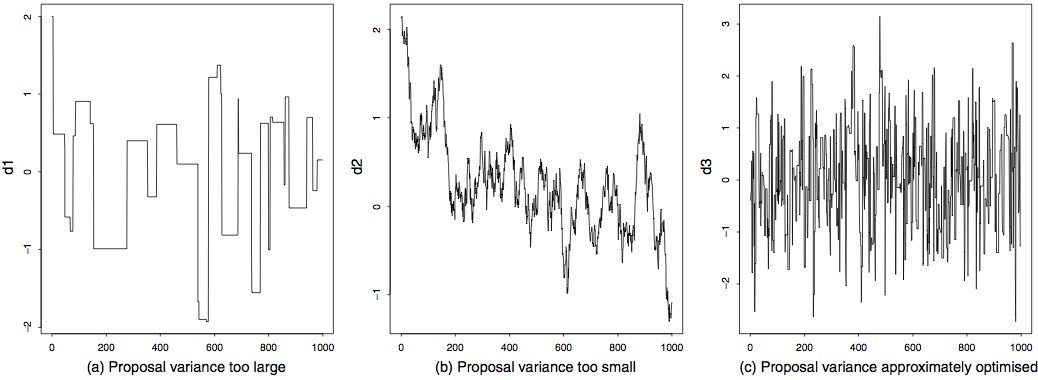
\includegraphics[width=0.85\textwidth]{img/roberts-rosenthal-traceplots.jpg}
\end{center}
\item \emph{Traceplots} show parameter value on $y$ axis, iterations on $x$
\item Empirical tuning problem; theoretical optima exist for some
  cases
\end{itemize}
\vfill\hfill
{\tiny Roberts and Rosenthal (2001) Optimal Scaling for Various
  Metropolis-Hastings Algorithms. {\slshape Statistical Science}.}


\sld{Convergence}
\begin{itemize}
\item Imagine releasing a hive of bees in a sealed house
\begin{subitemize}
\item they disperse, but eventually reach equilibrium where the same
  number of bees leave a room as enter it (on average)
\end{subitemize}
\item May take many iterations for Markov chain to reach equilibrium
\end{itemize}

\sld{Convergence: Example}
\begin{center}
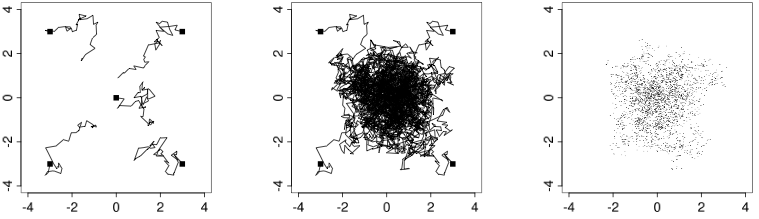
\includegraphics[width=0.8\textwidth]{img/bda-diffuse-converge.png}
\end{center}
\begin{itemize}
\item Four chains with different starting points
\begin{subitemize}
\item \emph{Left}: 50 iterations
\item \emph{Center}: 1000 iterations
\item  \emph{Right}: Draws from second half of each chain
\end{subitemize}
\vfill\hfill {\footnotesize Gelman et al., {\slshape Bayesian Data Analysis}}
\end{itemize}


\sld{Potential Scale Reduction ($\hat{R}$)}
\begin{itemize}
\item Gelman \& Rubin recommend $M$ chains of $N$ draws with
  \myemph{diffuse initializations}
\item Measure that each chain has same posterior mean and variance
\item If not, may be stuck in multiple modes or just not converged yet
\item Define statistic $\hat{R}$ of chains s.t. \myemph{at convergence},
$\hat{R} \rightarrow 1$
\begin{subitemize}
\item $\hat{R} >\!> 1$ implies non-convergence
\item $\hat{R} \approx 1$ \myemph{does not guarantee convergence}
\item Only measures marginals
\end{subitemize}
\end{itemize}

\sld{Split $\hat{R}$}
\begin{itemize}
\item Vanilla $\hat{R}$ may not diagnose non-stationarity
\begin{subitemize}
\item e.g., a sequence of chains with an increasing parameter
\end{subitemize}
\item \myemph{Split $\hat{R}$}: \ Stan splits each chain into first and
  second half
\begin{subitemize}
\item start with $M$ Markov chains of $N$ draws each
\item split each in half to creates $2M$ chains of $N/2$ draws
\item then apply $\hat{R}$ to the $2M$ chains
\end{subitemize}
\end{itemize}


\sld{Calculating $\hat{R}$ Statistic: Between}
\begin{itemize}
\item $M$ chains of $N$ draws each
\item \myemph{Between-sample variance} estimate
\[
B
= \frac{N}{M-1} \, \sum_{m=1}^M (\bar{\theta}^{(\bullet)}_{m} - \bar{\theta}^{(\bullet)}_{\bullet})^2,
\]
%
where
%
\[
\bar{\theta}_m^{(\bullet)}
= \frac{1}{N} \sum_{n = 1}^N \theta_m^{(n)}
\ \ \ \ \
\mbox{and}
\ \ \ \ \
\bar{\theta}^{(\bullet)}_{\bullet}
= \frac{1}{M} \, \sum_{m=1}^M \bar{\theta}_m^{(\bullet)}.
\]
\end{itemize}

\sld{Calculating $\hat{R}$ (cont.)}
\begin{itemize}
\item $M$ chains of $N$ draws each
\item \myemph{Within-sample variance} estimate:
\[
W 
= \frac{1}{M} \, \sum_{m=1}^M s_m^2,
\]
where
\[
s_m^2 = \frac{1}{N-1} \, \sum_{n=1}^N (\theta^{(n)}_m - \bar{\theta}^{(\bullet)}_m)^2.
\]
\end{itemize}

\sld{Calculating $\hat{R}$ Statistic (cont.)}
\begin{itemize}
\item \myemph{Variance} estimate:
\[
\widehat{\mbox{var}}^{+}\!(\theta|y)
= \frac{N-1}{N}\, W \, + \, \frac{1}{N} \, B.
\]
\\[4pt]
recall that $W$ is within-chain variance and $B$ between-chain
%
\vspace*{6pt}
\item \myemph{Potential scale reduction} statistic (``R hat'')
\[
\hat{R} 
\, = \,
\sqrt{\frac{\widehat{\mbox{var}}^{+}\!(\theta|y)}{W}}.
\]
\end{itemize}


\sld{Correlations in Posterior Draws}
%
\begin{itemize}
\item Markov chains typically display autocorrelation in the series of
  draws $\theta^{(1)}, \ldots, \theta^{(m)}$
\item Without i.i.d. draws, central limit theorem \emph{does not apply}
\item Effective sample size $N_{\mbox{\footnotesize eff}}$ divides out
  autocorrelation
\item $N_{\mbox{\footnotesize eff}}$ must be estimated from sample
\begin{subitemize}
\item Fast Fourier transform computes correlations at all lags
\end{subitemize}
\vspace*{-6pt}
\item Estimation accuracy proportional to 
{\large
\[
\frac{1}{\sqrt{N_{\mbox{\small eff}}}}
\]
}
\end{itemize}

\sld{Reducing Posterior Correlation}
\begin{itemize}
\item Tuning algorithm parameters to ensure good mixing
\item Recall Metropolis traceplots of Roberts and Rosenthal:
\begin{center}
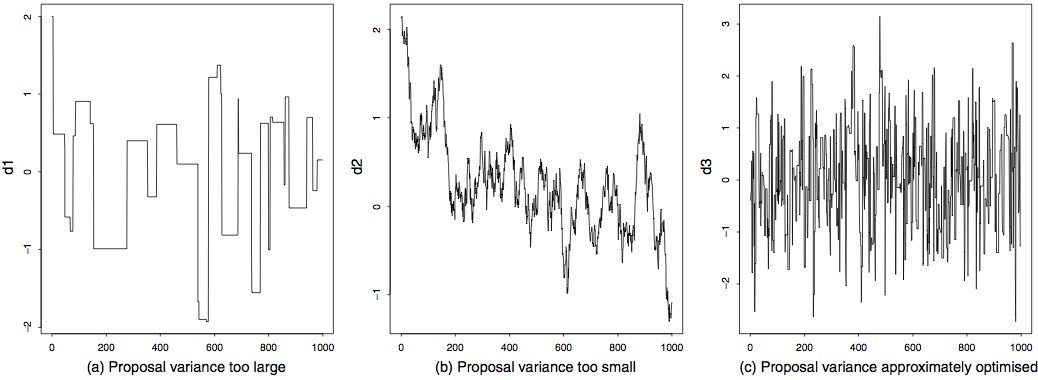
\includegraphics[width=0.85\textwidth]{img/roberts-rosenthal-traceplots.jpg}
\end{center}
\item Good jump scale $\sigma$ produces good mixing and high
$N_{\mbox{\footnotesize eff}}$
\end{itemize}


\sld{Effective Sample Size}
%
\begin{itemize}
\item Autocorrelation at lag $t$ is correlation between subseqs
\begin{subitemize}
\item $(\theta^{(1)},\ldots, \theta^{(N-t)})$ and $(\theta^{(1 + t)}, \ldots, \theta^{(N)})$
\end{subitemize}
\item  Suppose chain has density $p(\theta)$ with
\begin{subitemize}
\item $\mathbb{E}[\theta] = \mu$ \ \ and \ \ $\mbox{\rm Var}[\theta] = \sigma^2$ 
\end{subitemize}
\item Autocorrelation $\rho_t$ at lag $t \geq 0$:
\[
\rho_t  =  \frac{1}{\sigma^2} \, \int_{\Theta} (\theta^{(n)} - \mu)
       (\theta^{(n+t)} - \mu) \, p(\theta) \, d\theta
\]
\item Because $p(\theta^{(n)}) = p(\theta^{(n+t)}) = p(\theta)$ at convergence,
\[
\rho_t = \frac{1}{\sigma^2} \, \int_{\Theta} \theta^{(n)} \, \theta^{(n+t)} \, p(\theta) \, d\theta
\]
\end{itemize}

\sld{Estimating Autocorrelations}
\begin{itemize}\small
\item Effective sample size ($N$ draws in chain) is defined by
\[
N_{\mbox{\scriptsize eff}}
\ = \
\frac{N}{\sum_{t = -\infty}^{\infty} \rho_t}
\ = \
\frac{N}{1 + 2 \sum_{t = 1}^{\infty} \rho_t}
\]
\item Estimate in terms of variograms ($M$ chains) at lag $t$
\begin{subitemize}
\item Calculate with fast Fourier transform (FFT)
\end{subitemize}
\[
V_t = 
\frac{1}{M}
\,
\sum_{m=1}^M 
\
\left(
\frac{1}{N_m - t}
\sum_{n=t+1}^{N_m}
\left(
\theta_m^{(n)} - \theta_m^{(n-t)}
\right)^2
\right)
\]
\item Adjust autocorrelation at lag $t$ using cross-chain variance
  as
\[
\hat{\rho}_t
= 1 - \frac{\displaystyle V_t}{
            \displaystyle 2 \, \widehat{\mbox{var}}^{+}}
\]
\item If not converged, $\widehat{\mbox{var}}^{+}$ overestimates variance
\end{itemize}

\sld{Estimating $N_{\normalsize eff}$}
\begin{itemize}
\item Let $T'$ be first lag s.t.\ $\rho_{T' + 1} < 0$, 
\item Estimate autocorrelation by
\[
\hat{N}_{\mbox{\scriptsize eff}}
= 
\frac{MN}
     {1 + \sum_{t=1}^{T'} \hat{\rho}_t}.
\]
\item NUTS avoids negative autocorrelations, so first negative
  autocorrelation estimate is reasonable
\vfill
\item 
{\footnotesize For basics (not our estimates), see \\
Charles Geyer (2013) Introduction to MCMC. In
    {\slshape Handbook of MCMC}.
\\
(free online at \url{http://www.mcmchandbook.net/index.html})}
\end{itemize}


\sld{Gibbs Sampling}
\begin{itemize}
\item Draw random initial parameter vector $\theta^{(1)}$ (in
  support) 
\item For $m \in \range{2}{M}$
\begin{subitemize}
\item For $n \in \range{1}{N}$:
\begin{itemize}
\item draw 
$\theta^{(m)}_n$ according to conditional \\[8pt]
$p(\theta_n|\theta_1^{(m)},\ldots,\theta_{n-1}^{(m)}, \, \theta_{n+1}^{(m-1)},
\ldots,\theta_N^{(m-1)},  y)$.
\end{itemize}
\end{subitemize}
\item e.g, with $\theta = (\theta_1,\theta_2,\theta_3)$:
\begin{subitemize}
\item draw \ $\theta_1^{(m)}$  \ according to \ $p(\theta_1 | \theta_2^{(m-1)},
  \theta_3^{(m-1)}, y)$
\item draw \ $\theta_2^{(m)}$ \ according to \ $p(\theta_2 | \theta_1^{(m)},
  \theta_3^{(m-1)}, y)$
\item draw \ $\theta_3^{(m)}$ \ according to \ $p(\theta_3 | \theta_1^{(m)},
  \theta_2^{(m)}, y)$
\end{subitemize}
\end{itemize}

\sld{Generalized Gibbs}
\begin{itemize}
\item ``Proper'' Gibbs requires conditional Monte Carlo draws
\begin{subitemize}
\item typically works only for conjugate priors
\end{subitemize}
\item In general case, may need to use less efficient conditional
  draws
\begin{subitemize}
\item Slice sampling is a popular general technique that works for
  discrete or continuous $\theta_n$ (JAGS)
\item Adaptive rejection sampling is another alternative (BUGS)
\item Very difficult in more than one or two dimensions
\end{subitemize}
\end{itemize}

\sld{Sampling Efficiency}
\begin{itemize}
\item We care only about $N_{\mbox{\footnotesize eff}}$ per second
\item Decompose into
{\small
\begin{enumerate}
\item Iterations per second
\item Effective sample size per iteration
\end{enumerate}
}
\item Gibbs and Metropolis have high iterations per second (especially
  Metropolis)
\item But they have low effective sample size per iteration (especially
  Metropolis) 
\item Both are particular weak when there is high correlation among
  the parameters in the posterior
\end{itemize}

\sld{Hamiltonian Monte Carlo \& NUTS}
\begin{itemize}
\item Slower iterations per second than Gibbs or Metropolis
\item Much higher effective sample size per iteration for
complex posteriors (i.e., high curvature and correlation)
\item Overall, much higher $N_{\mbox{\footnote eff}}$ per second
\vfill
\item Details in the next talk \ldots
\item Along with details of how Stan implements HMC and NUTS
\end{itemize}

\mypart{}{The End (Section 3)}



\end{document}